\section{Result}

\begin{figure}[htbp]
    \centering
    \begin{subfigure}{0.4\textwidth}
        \centering
        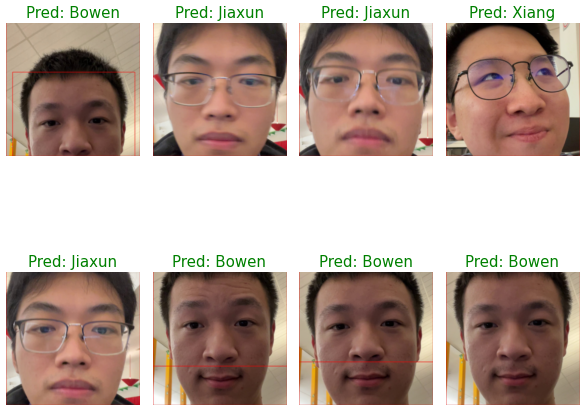
\includegraphics[width=1\textwidth]{pred_orig.png}
        \caption{Prediction without attack}
    \end{subfigure}
    \qquad
    \begin{subfigure}{0.4\textwidth}
        \centering
        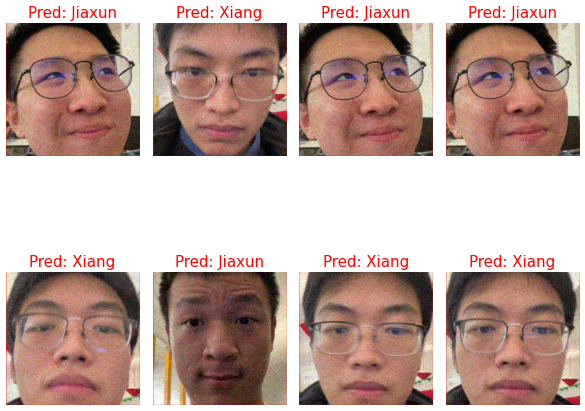
\includegraphics[width=1\textwidth]{pred_pgd_n.png}
        \caption{Prediction with non-targeted attack}
    \end{subfigure}
    \caption{Example of a non-targeted attack}
    \label{fig:pdf_attack_example}
\end{figure}

We can generate an adversarial example using the method described in the preceding steps. In the figure \ref{fig:pdf_attack_example}, the image on the left demonstrates that Resnet-18 correctly predicted the original photos. After adding the PGD model's generated noise. The image on the right depicts Resnet-18 classifying the adversarial example as a different category. We also generated perturbations on the test set with both targeted and non-targeted attack. Experimental results show that with either adversarial attack method, we achieved less than 5 percent accuracy, demonstrating the effectiveness of our adversarial attack. Thus, we can confidently say that our facial encryption can efficiently protect the users' privacy.  


